% 4-bit ripple carry annotated with propagation delay
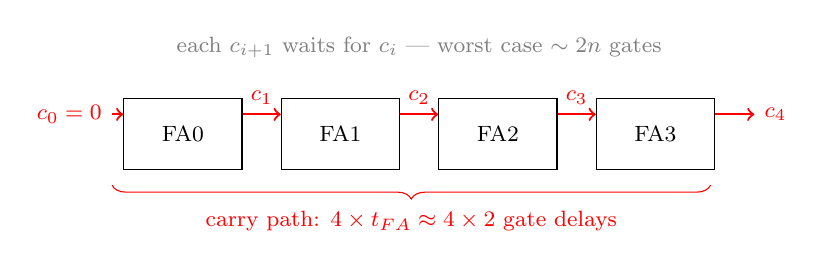
\begin{tikzpicture}[font=\footnotesize, cell/.style={draw, minimum width=1.5cm, minimum height=0.9cm}]
\node[cell] (f0) at (0,0) {FA0};
\node[cell] (f1) at (2,0) {FA1};
\node[cell] (f2) at (4,0) {FA2};
\node[cell] (f3) at (6,0) {FA3};
\draw[->, red, thick] (-0.9,0.25) node[left] {$c_0=0$} -- (f0.west|-0,0.25);
\draw[->, red, thick] (f0.east|-0,0.25) -- node[above] {$c_1$} (f1.west|-0,0.25);
\draw[->, red, thick] (f1.east|-0,0.25) -- node[above] {$c_2$} (f2.west|-0,0.25);
\draw[->, red, thick] (f2.east|-0,0.25) -- node[above] {$c_3$} (f3.west|-0,0.25);
\draw[->, red, thick] (f3.east|-0,0.25) -- ++(0.5,0) node[right] {$c_4$};
\draw[red, decorate, decoration={brace, mirror, amplitude=5pt}] (-0.9,-0.65) -- (6.7,-0.65)
  node[midway, below=6pt] {carry path: $4\times t_{FA}\approx 4\times 2$ gate delays};
\node[gray] at (3,1.1) {each $c_{i+1}$ waits for $c_i$ — worst case $\sim2n$ gates};
\end{tikzpicture}
